% !TeX root = ../main.tex
% ---------------------------------------------------------------
\section{Results}
\label{sec:results}
% ---------------------------------------------------------------

\subsection{Coverage and matching}

Of the \NOaEligible{} eligible OpenAlex authors, \NRankedPubvFrac{} have at least five works with a publication score and \NRankedCvFracNs{} have at least five works cited by scored works once self-citations are removed. Restricting citations to those made in 2025 leaves \NRankedCvFracSinglens{} researchers with a single-year citer score. Researchers drop out of a score when fewer than five of their works carry it, which happens when most of their papers appear in sources that are not retained in any field ranking or attract no citations from retained sources.

The matching procedure of Section~\ref{sec:data} assigned an OpenAlex author to \NMatchMatched{} of the \NStPersons{} Stanford persons, covering \NMatchCareerPct{}\% of the career table and \NMatchSinglePct{}\% of the single-year table. The single-year table matches less well. It contains more researchers who began publishing recently (16\% with a first paper in 2012 or later, against 2\% in the career table), whose short records make the volume comparison less discriminating, and its researchers who are not also in the career table have no comparable $h$-index, so their candidates are checked on paper count only. In a hand check of 100 randomly drawn matches, 98 agreed in name, in institution or country, and in paper count and $h$-index. The other two were common English names without an institutional match, which we could neither confirm nor reject. Of the remaining persons, \NMatchUnmatched{} had no candidate that agreed on surname, given name, country and volume, \NMatchImplausible{} had a best candidate identified only by initials and without an institutional match, \NMatchAmbiguous{} had two candidates of similar strength, and \NMatchConflict{} lost their candidate to a stronger claim by another Stanford person.

\subsection{Distribution of researcher scores}

Figure~\ref{fig:distributions} shows the distribution of the fractional scores. The median publication score of eligible researchers is \NMedPubAll{}, and \NSharePubAboveOneAll{}\% of them score above one. Stanford-listed researchers score higher, with a median of \NMedPubSt{} and \NSharePubAboveOneSt{}\% above one. The citer score is centred higher, with medians of \NMedCitAll{} for all eligible researchers and \NMedCitSt{} for Stanford-listed researchers, because the citing works that carry a score are those in retained sources, which on average have higher influence than the sources excluded from the ranking. The citer score is therefore a relative measure. Its value of one does not mark the field average in the way that $v = 1$ does for sources and institutions.

\begin{figure}[t]
\centering
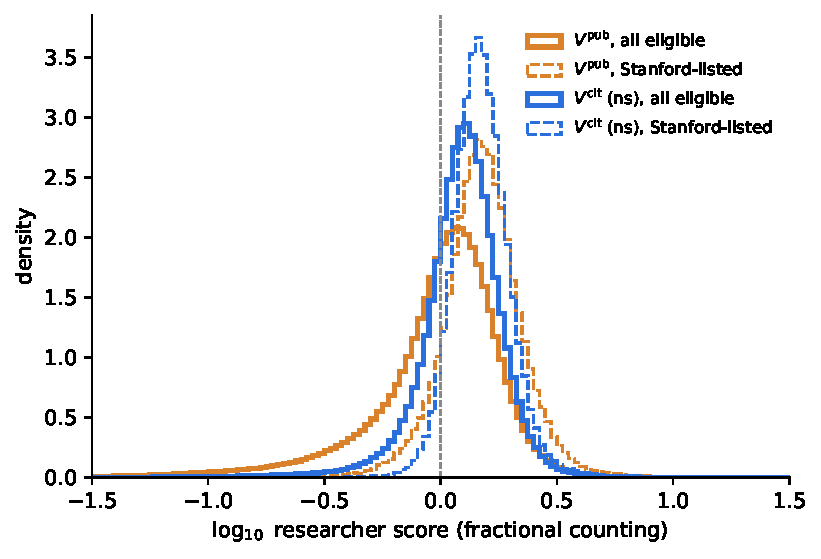
\includegraphics[width=0.7\textwidth]{figures/fig_distributions.pdf}
\caption{Distribution of researcher scores under fractional counting for all eligible OpenAlex researchers (solid) and for researchers matched to the Stanford career table (dashed). Citer scores exclude self-citations. The dashed vertical line marks a score of one.}
\label{fig:distributions}
\end{figure}

\subsection{Agreement with the Stanford indicators}

Among matched researchers, spectral scores and Stanford indicators are only weakly related (Table~\ref{tab:agreement}, Figure~\ref{fig:v_vs_c}). The Spearman correlation between the fractional publication score and $c$ is \NRhoPubfracC{}, and between the fractional citer score without self-citations and $c$ without self-citations it is \NRhoCitfracnsCns{}. Correlations with total citations and with $h$ are lower again, and correlations with the co-authorship-adjusted $h_m$ are close to 0.14 for every score. The single-year scores agree less with the single-year table than the career scores do with the career table.

Two features of the comparison keep these correlations low, and they should not be read as disagreement about the same quantity. The first is range restriction. The matched researchers are all in the top 2\% of their subfield or the top 100,000 by $c$, so the comparison is made within a narrow upper band of the $c$ distribution. The second, and more important, is that $c$ is cumulative and the spectral scores are means. When Stanford's citations are divided by papers to give a size-independent rate, the correlation with the fractional citer score rises to \NRhoCitfracnsNcpp{}, and with the fractional publication score to \NRhoPubfracNcpp{}. Within Stanford fields (Table~\ref{tab:fields}), the correlation of the citer score with $c$ ranges from \NFieldRhoMin{} in \NFieldMin{} to \NFieldRhoMax{} in \NFieldMax{}. The low value in physics is probably related to the exclusion of papers with 30 or more authors from the OpenAlex corpus, which removes much of the citation record on which $c$ rests in parts of that field.

\begin{table}[t]
\centering
\caption{Spearman correlations between spectral researcher scores and Stanford indicators for matched researchers with at least five contributing works. Career scores are compared with the career table and single-year (2025) citer scores with the single-year table. ``pub'' is the publication score, ``cit'' the citer score, ``ns'' excludes self-citations, and ``full'' and ``frac'' denote full and fractional counting. Stanford indicators include self-citations except for $c$ (ns).}
\label{tab:agreement}
\small
% generated by researchers/compare_stanford.py
\begin{tabular}{lrrrrrr}
\toprule
Spectral score & $c$ & $c$ (ns) & $n_c$ & $h$ & $h_m$ & $N$ \\
\midrule
pub, full & 0.32 & 0.36 & 0.33 & 0.25 & 0.13 & 196{,}223 \\
pub, frac & 0.32 & 0.37 & 0.32 & 0.25 & 0.14 & 196{,}223 \\
cit, full & 0.28 & 0.30 & 0.23 & 0.17 & 0.14 & 196{,}909 \\
cit, frac & 0.27 & 0.30 & 0.22 & 0.16 & 0.14 & 196{,}909 \\
cit, full, ns & 0.26 & 0.28 & 0.19 & 0.14 & 0.13 & 196{,}791 \\
cit, frac, ns & 0.25 & 0.27 & 0.18 & 0.13 & 0.13 & 196{,}791 \\
\midrule
cit 2025, full $\to$ single-yr & 0.23 & 0.25 & 0.11 & 0.12 & 0.15 & 184{,}419 \\
cit 2025, frac $\to$ single-yr & 0.22 & 0.24 & 0.10 & 0.11 & 0.16 & 184{,}419 \\
cit 2025, full, ns $\to$ single-yr & 0.22 & 0.24 & 0.08 & 0.10 & 0.15 & 184{,}292 \\
cit 2025, frac, ns $\to$ single-yr & 0.22 & 0.23 & 0.07 & 0.09 & 0.16 & 184{,}292 \\
\bottomrule
\end{tabular}

\end{table}

\begin{figure}[t]
\centering
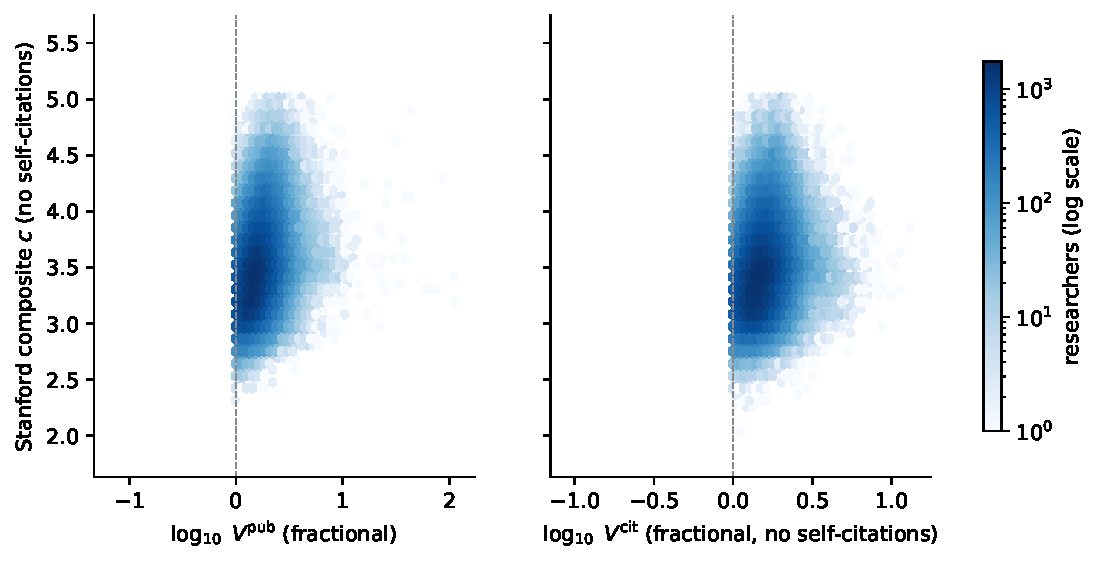
\includegraphics[width=\textwidth]{figures/fig_v_vs_c.pdf}
\caption{Stanford composite indicator $c$ without self-citations against the fractional publication score (left) and the fractional citer score without self-citations (right), for matched researchers in the career table. Shading is the number of researchers on a logarithmic scale.}
\label{fig:v_vs_c}
\end{figure}

\begin{table}[t]
\centering
\caption{Spearman correlations by Stanford field (main field of the researcher) for matched career-table researchers with at least five cited works. The last column compares the citer score with Stanford citations per paper, excluding self-citations. Fields with fewer than 200 matched researchers are omitted.}
\label{tab:fields}
\small
\resizebox{\textwidth}{!}{% generated by researchers/compare_stanford.py
\begin{tabular}{lrrrr}
\toprule
Stanford field & $N$ & $V^{\mathrm{pub}}$ vs $c$ & $V^{\mathrm{cit}}_{\mathrm{ns}}$ vs $c$ (ns) & $V^{\mathrm{cit}}_{\mathrm{ns}}$ vs $n_c/n_p$ (ns) \\
\midrule
Agriculture, Fisheries \& Forestry & 6{,}891 & 0.17 & 0.18 & 0.34 \\
Biology & 8{,}099 & 0.36 & 0.38 & 0.49 \\
Biomedical Research & 16{,}091 & 0.33 & 0.28 & 0.45 \\
Built Environment \& Design & 1{,}227 & 0.25 & 0.23 & 0.09 \\
Chemistry & 12{,}972 & 0.24 & 0.27 & 0.38 \\
Clinical Medicine & 62{,}899 & 0.29 & 0.23 & 0.39 \\
Communication \& Textual Studies & 873 & 0.41 & 0.36 & 0.38 \\
Earth \& Environmental Sciences & 6{,}795 & 0.26 & 0.26 & 0.37 \\
Economics \& Business & 3{,}871 & 0.26 & 0.20 & 0.52 \\
Enabling \& Strategic Technologies & 15{,}873 & 0.25 & 0.22 & 0.43 \\
Engineering & 14{,}649 & 0.29 & 0.29 & 0.38 \\
Historical Studies & 772 & 0.36 & 0.22 & 0.32 \\
Information \& Communication Technologies & 14{,}251 & 0.27 & 0.26 & 0.42 \\
Mathematics \& Statistics & 2{,}266 & 0.18 & 0.27 & 0.50 \\
Philosophy \& Theology & 390 & 0.37 & 0.38 & 0.35 \\
Physics \& Astronomy & 16{,}856 & 0.18 & 0.13 & 0.24 \\
Psychology \& Cognitive Sciences & 3{,}466 & 0.20 & 0.14 & 0.35 \\
Public Health \& Health Services & 3{,}879 & 0.46 & 0.42 & 0.32 \\
Social Sciences & 4{,}627 & 0.29 & 0.29 & 0.42 \\
\bottomrule
\end{tabular}
}
\end{table}

\subsection{Two top-2\% lists}

Drawing up a top-2\% list within each OpenAlex subfield on spectral scores produces a list that overlaps little with Stanford's (Table~\ref{tab:top2}). Only \NTopInStCitfracns{}\% of the \NTopNCitfracns{} researchers in the top 2\% by the fractional citer score without self-citations appear in the Stanford career table, and only \NStInTopCitfracns{}\% of matched Stanford researchers are in that top 2\%. The publication score overlaps more, at \NTopInStPubfrac{}\% and \NStInTopPubfrac{}\% respectively. The difference lies in volume. The median top-2\% researcher by citer score has \NTopMedWorksCit{} eligible works in the corpus and \NTopMedCitesCit{} non-self citations, against \NStMedWorks{} works and \NStMedCites{} citations for the median matched Stanford researcher. A mean rewards a short record of papers cited by influential sources, whereas $c$ rewards a long record of many citations, and the two lists select largely different people.

\begin{table}[t]
\centering
\caption{Top-2\% lists formed within OpenAlex subfields on each spectral score. ``\% on Stanford list'' is the share of the spectral top 2\% matched to a researcher in the Stanford career table, a lower bound because some Stanford researchers are not matched. The last column is the share of matched Stanford researchers who fall in the spectral top 2\%.}
\label{tab:top2}
\small
% generated by researchers/compare_stanford.py
\begin{tabular}{lrrr}
\toprule
Spectral score & Top 2\% (OA subfield) & \% on Stanford list & \% of matched Stanford in top 2\% \\
\midrule
pub, full & 148{,}659 & 7.9 & 6.0 \\
pub, frac & 148{,}659 & 9.2 & 6.9 \\
cit, full & 139{,}623 & 3.4 & 2.4 \\
cit, frac & 139{,}623 & 3.5 & 2.4 \\
cit, full, ns & 134{,}779 & 3.0 & 2.1 \\
cit, frac, ns & 134{,}779 & 3.1 & 2.1 \\
\bottomrule
\end{tabular}

\end{table}

The country composition of the lists also differs (Table~\ref{tab:countries}). The United States accounts for \NShareUsAll{}\% of eligible researchers, \NShareUsSt{}\% of the Stanford career list, \NShareUsCit{}\% of the top 2\% by citer score and \NShareUsPub{}\% of the top 2\% by publication score. China accounts for \NShareCnAll{}\% of eligible researchers but \NShareCnSt{}\% of the Stanford list, \NShareCnCit{}\% of the citer-score list and \NShareCnPub{}\% of the publication-score list. The publication score, which depends on the influence of a researcher's journals and institutions, concentrates the list in the United States more strongly than any citation-based list. Australia accounts for \NShareAuAll{}\% of eligible researchers, \NShareAuSt{}\% of the Stanford list, and \NShareAuCit{}\% and \NShareAuPub{}\% of the two spectral lists. Of the \NAuEligible{} eligible researchers whose last known institution is Australian, \NAuTopCitfracns{} are in the top 2\% of their subfield by citer score and \NAuTopPubfrac{} by publication score, against \NAuStCareer{} Australian entries in the Stanford career table.

\begin{table}[t]
\centering
\caption{Country shares (\%) of the Stanford career list, of the spectral top-2\% lists, and of all eligible OpenAlex researchers, for the twelve countries with the most Stanford-listed researchers. Countries are the researcher's most recent country in each database.}
\label{tab:countries}
\small
% generated by researchers/compare_stanford.py
\begin{tabular}{lrrrr}
\toprule
Country & Stanford career list & $V^{\mathrm{pub}}$ frac & $V^{\mathrm{cit}}$ frac, ns & All eligible \\
\midrule
US & 37.3 & 58.4 & 41.6 & 17.1 \\
GB & 8.8 & 9.0 & 6.8 & 3.6 \\
CN & 6.0 & 5.0 & 8.9 & 18.1 \\
DE & 5.3 & 4.0 & 6.3 & 3.6 \\
CA & 4.1 & 2.2 & 3.2 & 2.3 \\
JP & 3.7 & 0.7 & 3.1 & 4.2 \\
AU & 3.5 & 1.4 & 2.0 & 1.8 \\
FR & 3.1 & 2.0 & 3.9 & 2.8 \\
IT & 3.0 & 0.7 & 1.7 & 2.8 \\
NL & 2.1 & 2.5 & 2.2 & 1.2 \\
ES & 1.7 & 0.8 & 1.6 & 2.5 \\
IN & 1.6 & 0.4 & 0.8 & 4.0 \\
\bottomrule
\end{tabular}

\end{table}

\subsection{Self-citation and counting}

The self-citation shares measured in the two databases agree closely. For matched researchers with at least 50 citations, the Spearman correlation between the OpenAlex self-citation share and Stanford's is \NSelfRho{}, and the medians are \NSelfMedOurs{}\% and \NSelfMedSt{}\%. Across all eligible researchers with at least 50 citations the median is \NSelfMedAll{}\%, and \NSelfOverFortyPct{}\% have more than 40\% self-citations, against \NStSelfOverFortyPct{}\% of the Stanford career list.

Removing self-citations changes the citer score little. The Spearman correlation between the fractional citer scores with and without self-citations is \NRhoCitAllNs{}, and the median researcher moves by \NSelfShiftMed{} percentile points (90th percentile \NSelfShiftNinety{}). For researchers with more than 40\% self-citations, removing them raises the median percentile by \NSelfHiGain{} points rather than lowering it. For these researchers the self-citing papers sit, on average, in sources of lower influence than the papers of their other citers, so removing them raises the mean. A citer score cannot be raised by self-citation unless the self-citing papers appear in sources more influential than those of the researcher's other citers.

The choice between full and fractional counting matters even less. The Spearman correlation between full and fractional scores is \NRhoPubFullFrac{} for the publication score and \NRhoCitFullFrac{} for the citer score. Because both scores are means rather than sums, fractional counting changes only the relative weight of a researcher's own papers, which matters only when their author counts vary widely. The career and single-year citer scores correlate at \NRhoCitCareerSingle{}.
